
%% ==============
\chapter{Photon-based Next Event Estimation}
\label{ch:PNEE}
%% ==============

We propose a novel approach to find estimators for importance sampling (especially) for scenes with many localized light sources. Our key goal is to efficiently reduce the variance $\sigma$ (section~\ref{sec:IS})\pdfcomment{ref to sections?} of the direct lighting term of our Monte Carlo integrator (section~\ref{sec:MC}) by estimating the strength of the light contribution from every light source. Typically ruling out light sources that contribute nothing (zero contribution paths) due to shadowing has a significant impact.

In a preprocess all light sources scatter out photons into the scene, similar to photon mapping \cite{jensen2001realistic}, but no bounces are considered, as we only need direct light paths for our Next Event Estimation estimator. Further, we only consider LD paths, all LS*D paths are disregarded. Those paths are disregarded by the first condition anyway, but we want to emphasize that refractions of any kind make a photon obsolete for our usecase. After the photons are scattered out into the scene we are looking for efficient ways to approximate or store those photons. Contrary to techniques like proposed by \cite{Estevez} where we build up our datastructures around the light sources themselves, with PNEE we build the datastructures around the light-receiving parts of our scene. This generally will scale up the data that needs to be processed but at the same time bear opportunity to refine our estimators. Then, the last step happens from within our pathtracer, we produce an estimator for our Next Event Estimation at every intersection by accessing and processing surrounding photons or CDFs.

Note that when the photon count goes towards infinity and the intersection search radius goes towards zero the estimator becomes the direct lighting term we are trying to find, making the Monte Carlo integration obsolete. As we are bound by time and memory, the key challenge is to find a good approximation thereof in minimal time. We found that shooting, processing and storing photons in the preprocess is not as tightly bound, but the lookup thereof in the integrator is very timecritical as it runs once for each intersection in the pathtracer. In the following sections we discuss various datastructures and storing methods we explored throughout this work.

% TODO introduce mix and match here already? Or at least point out the structure

\section{Shooting photons}

power based sampling ...

calculation of beta ...


\section{Form of storage}

\subsection{Photons}

Storing every photon with its weight and potentially additional data like the direction it came from is the most precise form to later compute our estimator, as the number of datapoints corresponds to our photon count. For every intersection point we evaluate the surrounding photons and compute an individual cumulative distribution function. As the photon count is quite high, typically several million unevenly distributed datapoints, the lookup is a bottleneck in this case, even with acceleration structures like a k-d tree that we discuss in section~\ref{sec:pneekdtree}. Nonetheless, the approach is worthwhile due to the potential quality of the estimator.

\subsection{Lightcut}

If we want to lessen the strain on the integrator, we might reduce the number of datapoints within the preprocess and store an approximation instead of every photon. Recent work from Estevez and Kulla \cite{Estevez} and Vévoda and Křivánek \cite{Vevoda} rely on lightcuts. A lightcut is a horizontal cut through a lighttree (essentially a binary tree with light sources as leafs) and has the advantage of being very compact when many adjacent leafs of the subtree have the same sampling probability. This is quite typical, as most of the times only a small portion of lights contribute to a given point, while all other lights are shadowed. Let $n$ be the number of lights and $c$ the size of the cut. $c$ can be anything between one, cutting once at the root node, and $n$, cutting each leaf. Lightcuts thus adapt to the complexity of the given datapoint and often can be stored quite compact. Sampling from such a cut runs in $O(log n)$ but on avarage in $O(log c)$, size of the lighttree is $O(nlogn)$. The advantages of lightcuts break down when there are none or few adjacent samples that share the same probability. Proposed algorithms by Estevez \cite{Estevez} and others to find such a cut, in our view, have similarities to unsupervised machine learning algorithms, where the lighttree is a dendrogram of a cluster (typically produced by agglomerative hierarchical clustering) and the algorithm tries to assign a label (the probability) to the lights based on their cluster affinity. 

\subsection{CDF}

Another possibility is to directly store cumulative distribution functions during the preprocess. A CDF is usually stored as an sorted array of float values that grow from 0 to 1, the size is fixed at $n$, and sampling is done in $O(logn)$. With our technique we found lightcuts not well fitting, as rather than making broad approximate statements about clusters of lights, we dominantly have individually distinct contributions accumulated through photons. Let $k$ be the number of contributing light sources to a particular CDF, which equals to all light sources with a sampling probability unequal to zero. This would degenerate a lightcut into a CDF where $c \approx k$. Especially when creating CDFs within the integrator a linear space and timecomplexity is generally unacceptable. We observe that most of the time $k$ is significantly smaller than $n$ due to localized light influences. To address this issue we present Sparse CDFs in section~\ref{sec:sparse} where space- and time complexity for construction is $O(k)$ and sampling is $O(logk)$. Furthermore, in section \ref{sec:intcdf} we introduce the possibility to sublinearly interpolate between any kind of CDFs in $O(d)$ space and time for construction and $O(d + logn)$ sampling, where $d$ is the number of interpolated CDFs.
%TODO: Wie tief soll ich hier gehen wieso das so ist?

\subsubsection{Sparse CDF}
\label{sec:sparse}
\begin{figure}[htb] 
	\centering
	\begin{tikzpicture}[scale=7, cdf/.style ={thick}]

        
        %zoom lines
        \draw (0,0) -- (0,-0.2);
        \draw (1,0) -- (0.8,-0.2);
        

        %cdfs, lines and filling
        \draw[thick, fill=green!10] (0,0) rectangle (0.25, 0.1) node[pos=.5] {25\%};
        \draw[thick, fill=red!10] (0.25, 0) rectangle (0.5, 0.1) node[pos=.5] {25\%};
        \draw[thick, fill=blue!10] (0.5, 0) rectangle (1, 0.1) node[pos=.5] {50\%};
        
        \draw[thick, fill=green!10] (0, -0.3) rectangle (0.2, -0.2) node[pos=.5] {20\%};
        \draw[thick, fill=red!10] (0.2, -0.3) rectangle (0.4, -0.2) node[pos=.5] {20\%};
        \draw[thick, fill=blue!10] (0.4, -0.3) rectangle (0.8, -0.2) node[pos=.5] {40\%};
        
        \draw[thick, fill=black!10] (0.8, -0.3) rectangle (1, -0.2);
        
        \fill[fill=green!10] (0.84, -0.3) rectangle (0.86, -0.2);
        \fill[fill=red!10] (0.88, -0.3) rectangle (0.9, -0.2);
        \fill[fill=blue!20] (0.98, -0.3) rectangle (1, -0.2);
        
        \foreach\x in {0.82,0.84,...,0.98}
            \draw (\x,-0.2) -- (\x,-0.3);
            
        \draw[cdf] (0,0) rectangle node[left=4cm] {Inner CDF} (1,0.1);
        \draw[cdf] (0,-0.3) rectangle node[left=4cm] {Sparse CDF} (1,-0.2);
        
        % b range indicators
        \draw[thick] (0, -0.16) -- node[above] {$1-b = 0.8$} (0.8, -0.16) ;
        \draw[thick] (0, -0.17) -- (0, -0.15);
        
        \draw[thick] (0.8, -0.16) -- (1, -0.16) node[above] {$b = 0.2$} ;
        \draw[thick] (0.8, -0.17) -- (0.8, -0.15);
        \draw[thick] (1, -0.17) -- (1, -0.15);
        
        % braces
        \draw[line width=1.25pt, decoration={calligraphic brace,amplitude=7pt,mirror,raise=6pt},decorate]
                        (0,-0.3) -- node[below=12pt] {$k = 3$} (0.8,-0.3);
        \draw[line width=1.25pt, decoration={calligraphic brace,amplitude=7pt,mirror,raise=6pt},decorate]
                        (0.8,-0.3) -- node[below=12pt] {$n$} (1,-0.3);
        \draw[line width=1.25pt, decoration={calligraphic brace,amplitude=7pt,mirror,raise=26pt},decorate]
                        (0,-0.3) -- node[below=32pt] {$n$ distinct samples} (1,-0.3);

    \end{tikzpicture}
    \caption{A sparse CDF either samples from the uniform part with probability $b$ or from the inner CDF with probability $1-b$. $k$ are the number of samples that have a non-zero probability in the non-uniform part. All $k$ samples are repeated within the uniform part to facilitate calculations of $p_{sparse}$ (equation \ref{eq:psparse}). The samples in sparse CDF are not in the correct order, as a result two additional hashmaps are needed.} 
    \label{fig:sparseCDF}
\end{figure}

We need\pdfcomment{we need?} a CDF where only particular values from $0$ to $n$ may be sampled. We achieve this by using a classic CDF (inner CDF) with length $k$ and a hashmap which maps values $[1,k]\to [1,n]$\footnote{As the pre-image in $[1,k]\to [1,n]$ is a sequence this could also be a simple array instead of a hashmap. Before constructing the sparse CDF the photons are collected by some algorithm without knowing $k$ beforehand. As photons can originate from all $n$ light sources a hashmap is needed anyway. We continue with this hashmap to spare the conversion.}. After we sampled a number the map will map the sampled number to the original sample number. Further we also need a backmap which is the reverse of the former map. The backmap is used when you want to know the probability of a given original sample number $x$. The original sample number is mapped to the sample number that it corresponds to in the inner CDF, so the inner CDF can be queried for the corresponding probability. We additionally want to provide a base floor probability $b$, which is split equally by all $n$ light sources. Let $N$ be the set of all $n$ sample numbers and $K$ be the set of non-zero probability samples. The probability that a given sample $x$ is sampled by the sparse CDF is given as follows.
\begin{equation}\label{eq:psparse}
 p_{sparse}(x) = 
\begin{dcases}
    p_{inner}(backmap(x)) * (1 - b) + \frac{b}{n},& \text{if } x \in K\\
    \frac{b}{n}, & \text{otherwise}
\end{dcases}
\end{equation}
Even though we seemingly introduce unnecessary variance with this uniform base, it is absolutely crucial as we otherwise would introduce bias whenever our estimator would "forget" a light source, which is not uncommon for e.g. very distant or highly occluded light sources. Apart from that fact, it generally helps in areas where our estimator is bad for any reason, therefore the choice of $b$ should not be minimal, but rather roughly proportional to the expected quality of the estimator.

Construction is done in $O(k)$ space and time, sampling in $O(logk)$. Comparing to lightcuts we have a simpler datastructure in hand, that rules out non contributing light samples effectively. If we assume that equal non-zero probabilities are rare, which should be the case with many photon contributions, we generally should outperform lightcuts, especially because sampling the dominant case $x \notin K$ runs in $O(1)$. 

\subsubsection{Interpolated CDF}
\label{sec:intcdf}
\begin{figure}[htb] 
	\centering
	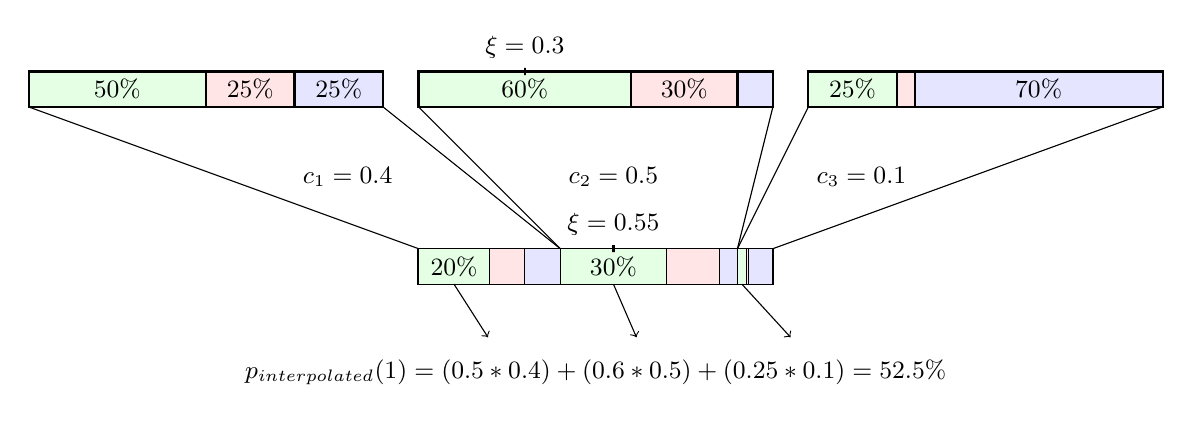
\begin{tikzpicture}[scale=4.5, cdf/.style ={thick}]
        \small
        %zoom lines
        \draw (-1.1,0) -- (0,-0.4);
        \draw (-0.1,0) -- (0.4,-0.4);
        \draw (0,0) -- (0.4,-0.4);
        \draw (1,0) -- (0.9,-0.4);
        \draw (1.1,0) -- (0.9,-0.4);
        \draw (2.1,0) -- (1,-0.4);
        
        \draw[cdf] (-1.1,0) rectangle (-0.1,0.1);
        \draw[cdf] (0,0) rectangle (1,0.1);
        \draw[cdf] (1.1,0) rectangle (2.1,0.1);
        \draw[cdf] (0,-0.5) rectangle (0.4,-0.4);
        \draw[cdf] (0.4,-0.5) rectangle (0.9,-0.4);
        \draw[cdf] (0.9,-0.5) rectangle (1,-0.4);
        
        %cdfs, lines and filling
        \draw[thick, fill=green!10] (-1.1,0) rectangle (-0.6, 0.1) node[pos=.5] {50\%};
        \draw[thick, fill=red!10] (-0.6, 0) rectangle (-0.35, 0.1) node[pos=.5] {25\%};
        \draw[thick, fill=blue!10] (-0.35, 0) rectangle (-0.1, 0.1) node[pos=.5] {25\%};
        
        \draw[thick, fill=green!10] (0,0) rectangle (0.6, 0.1) node[pos=.5] {60\%};
        \draw[thick, fill=red!10] (0.6, 0) rectangle (0.9, 0.1) node[pos=.5] {30\%};
        \draw[thick, fill=blue!10] (0.9, 0) rectangle (1, 0.1);
        
        \draw[thick, fill=green!10] (1.1,0) rectangle (1.35, 0.1) node[pos=.5] {25\%};
        \draw[thick, fill=red!10] (1.35, 0) rectangle (1.4, 0.1);
        \draw[thick, fill=blue!10] (1.4, 0) rectangle (2.1, 0.1) node[pos=.5] {70\%};
        
        \draw[fill=green!10] (0,-0.5) rectangle (0.2,-0.4) node[pos=.5] {20\%};
        \draw[fill=red!10] (0.2,-0.5) rectangle (0.3,-0.4);
        \draw[fill=blue!10] (0.3,-0.5) rectangle (0.4,-0.4);

        \draw[fill=green!10] (0.4,-0.5) rectangle (0.7,-0.4) node[pos=.5] {30\%};
        \draw[fill=red!10] (0.7,-0.5) rectangle (0.85,-0.4);
        \draw[fill=blue!10] (0.85,-0.5) rectangle (0.9,-0.4);
        
        \draw[fill=green!10] (0.9,-0.5) rectangle (0.925,-0.4);
        \draw[fill=red!10] (0.925,-0.5) rectangle (0.93,-0.4);
        \draw[fill=blue!10] (0.93,-0.5) rectangle (1,-0.4);
        
        \draw[thick] (0.55,-0.39) node[above] {$\xi = 0.55$} rectangle (0.55,-0.41);
        
        \draw[thick] (0.3, 0.11) node[above] {$\xi = 0.3$} rectangle (0.3,0.09);
        
        \node at (0.5, -0.75) {$p_{interpolated}(1) = \overbracket{(0.5 * 0.4)} + \overbracket{(0.6 * 0.5)} + \overbracket{(0.25 * 0.1)} = 52.5\%$};
        
        \draw[->] (0.1,-0.5) -- (0.196,-0.65);
        \draw[->] (0.55,-0.5) -- (0.615,-0.65);
        \draw[->] (0.9125,-0.5) -- (1.05,-0.65);
        
        % pi range indicators
        \path (-0.2, -0.25) node[above] {$c_1 = 0.4$};
        \path (0.55, -0.25) node[above] {$c_2 = 0.5$};
        \path (1.25, -0.25) node[above] {$c_3 = 0.1$};
        
    \end{tikzpicture}
    \caption{Three CDFs should be interpolated with corresponding weights $c_i$. Randomnumber $\xi$ is $0.55$. The second CDF is chosen, $\xi$ is cut and normalized to $0.3$. Sample 1 (green) is chosen. $p_{interpolated}$ is calculated according to equation \ref{eq:pinter}.} 
    \label{fig:interpolatedCDF}
\end{figure}

Suppose we want to sample a number from an interpolation between $d$ CDFs. A naive approach to achieve this is to loop through every CDF and for every sample add up the weights, normalize them in the end and store this as the new interpolated CDF. Construction would then run in $O(d * n)$ and $O(n)$ space, sampling in $O(logn)$. As we will need the construction to run for every intersection in our scene it is unsustainable to have it run linearly in $n$. We propose a CDF interpolation scheme that constructs in $O(d)$ time and space, with only minimal drawback when sampling with $O(d + logn)$.

We receive a list of CDFs to interpolate and corresponding weights. We loop through the weights and normalize them, thus constructing an usual CDF that will sample $i \in [1,d]$. We keep an array of references to the base CDFs. Now, for the lookup we sample $i$ in $O(logd)$ and then choose the $i'th$ CDF and sample within the CDF in $O(logn)$. We now have the sample $x$ and also have to calculate the probability that $x$ was sampled. Let $c_i$ be the probability to sample the $i'th$ CDF and $p_i(x)$ the probability of sampling $x$ within the $i'th$ CDF, we calculate the probability as follows.

\begin{equation}\label{eq:pinter}
    p_{interpolated}(x) = \sum_{i=1}^{d}p_{i}(x) * c_i
\end{equation}

The time complexity for this calculation is $O(d)$, resulting in overall complexity $O(logd + logn + d) = O(d + logn)$. The whole process is illustrated in figure \ref{fig:interpolatedCDF}. Note that with our construction all base CDFs are required to have the same number of samples $n$ in the exact same order. This restriction might be lifted with additional maps, similar to sparse CDFs, but we have no need for it, as all our used CDFs have the same $n$ lights, thus we spare the overhead.




\section{Acceleration datastructure}

After choosing what we store we are choosing how we store and access it from within our integrator. A critical part of finding our estimator is to access the data we previously stored. It is important to keep the probable distribution of photons in mind. Usually large parts of the scene won't have any photons and then there will be photon clusters, typically distributed on 3D-planes. Further, a typical problemcase for the choice of acceleration datastructures is called "teapot in a stadium" \pdfcomment{illustration?}. It describes the potentially vastly varying level of detail in a scene. The "teapot" is a small, highly detailed object in the "stadium" which is big, simple and mostly empty. This bears a typical trade off between adaptive datastructures like octrees or k-d trees, which handle varying LOD quite well, but generally have slower access times and static datastructures like a hashed grid, which has fast constant access times, but can't adapt to LOD at all. For our renderer often times not even the big O runtime is critical, but the constant overhead can be problematic, too. The best choice is often scene dependent, nonetheless, we are trying to find a good middleground that solves typical problem cases in photorealistic scenes. The form of storage does also impact the effectivness of the acceleration datastructure, we present natural fits in the following chapters.

\subsection{Hashed grid}

Storing photons directly into a hashed grid is quite dangerous, almost any scene will have clusters of photons, sometimes consisting of a large portion of the total photon count. When doing a nearest neighbour lookup of our intersection point this can degenerate to linear run time complexity, not even in the light source count $n$, but in the total photon count. It is apparent that this is unacceptable, as even a small detail in the scene could blow up rendering times.

The idea here is to store exactly one CDF in the middle of each grid cell and using the clamped position as the key. Doing so, we utilize the constant access times of the hashed grid without the threat of photon clusters. At the same time we are giving up precision, as we loose all positional data of the photons. We do not interpolate the photons by distance to the CDF, rather every photon contributes at the same rate to this homogeneous grid cell. As every intersection point will clearly choose one CDF, this leads to sometimes very apparent variance cliffs at the edges of the grid cells (see figure \ref{fig:varianceEdge}). PBRTs \cite{pbrt} and Vevodas \cite{Vevoda} \pdfcomment{use cite here or ref to the section where I introduced the technique?} technique have the exact same problem, but their CDFs transition somewhat smoothly as only position and angles are used for CDF calculation. The problem is highly accelerated with our technique because we inherit occlusion in the CDF generation which can create sharp edges in certain situations. We tackle this problem in section \ref{ch:trilinear}.


\subsection{k-d Tree}
\label{sec:pneekdtree}

\section{Interpolation}

\subsection{Trilinear interpolation}
\label{ch:trilinear}




\section{Mix and Match}

\section{Further Optimizations}



\subsection{Normal culling}






\section{Adaptive Parametrization}

\subsection{Photon Count}

\subsection{Adaptive importance weight}



